\chapter{Experiments and Results}

This chapter aims to outline the performed experiments on both datasets along with achieved results. In the discussion section, we interpret the results and explain what might be altered or improved in future experiments. Finally, we propose future experiments that may follow the present work.

\section{Finding the Optimal Model}

As described in the last chapter, we utilized Weights and Biases platform for a hyperparameter search. We hypothesized that the model’s performance is highly dependent on the number of orientations to which the network should be equivariant. As the readout is constrained to predict a neuron's response from just one scalar value, it needs to fetch the number from a relevant spatial position and a relevant orientation. The more orientations are available to choose from, the more specialized the features can potentially be, and thus the performance should increase. To investigate this hypothesis, each hyperparameter search has the number of orientations fixed, dividing the network architectures into groups determined by the training dataset and number of orientations to which the network should be equivariant. From now on, we will refer to these groups of networks as \emph{categories}. Moreover, with a higher number of orientations, the number of parameters in the core increases linearly, leading to a significant increase in the number of trainable parameters to be fit. This is another reason to search for hyperparameters separately for a distinct number of orientations.

The models were fitted by the Adam optimizer \citep{kingma2014adam} with an early stopping after 5 or 10 consecutive steps during which the correlation on the validation dataset did not improve (10 in the case of the Lurz et al. dataset \citep{lurz2021generalization}, 5 in case of the synthetic dataset). The batch size was set to 10. The model’s performance was evaluated by Pearson’s correlation on the validation dataset and was consequently used for comparing different choices of hyperparameters. The best-performing model was evaluated on the test set by Pearson’s correlation of the predicted responses with ten averaged responses to the same stimulus.

\section{Searched Hyperparameters}

An important parameter was the learning rate, which controls how strongly the gradient influences the weights’ update in each step. The next three hyperparameters were kernel sizes in the first layer, the last layer, and all other layers. Although the number of layers and channels in each convolutional layer are dependent variables, they were tuned independently of each other as the Weights and Biases platform does not yet support such a feature. The core's regularization strength factors in the first layer and the other layers were the next values to be found by the hyperparameter search. The proper way to initialize the network was learned by tuning the ranges of initial neurons' positions and by the parameter sigma describing the standard deviation of the Gaussian curve, from which the neurons' positions were sampled. Another question was whether to use depth-separable convolution or not, which was also decided based on the performance on the validation dataset.

\section{Control Model}

In the control model adapted from Lurz et al. \citep{lurz2021generalization}, all layers were regularized according to the original paper. Hyperparameter searches were done on each dataset separately to find the optimal network settings. In the following sections, this control model will indicate how much predictive precision was lost due to the bottleneck. 

Since our hyperparameter search is not as extensive as in the work of Lurz et al. \citep{lurz2021generalization}, the results are not as high. Moreover, our dataset is much more limited than the one used in the original paper. For this reason, achievable performance is likely higher. However, all trained networks had approximately similarly extensive search. If we devoted more time to parameter search of each network, the performances of all the networks in this work would likely grow proportionally, keeping the fraction of correlation intact. 

\section{Best Models Trained on Lurz et al. Dataset}\label{best_lurz_section}

We performed the hyperparameter searches for three fixed numbers of orientations; 8, 16, and 24. As hypothesized, the higher the number of rotations, the better the predictive performance of the best model. Along with the mentioned hyperparameters, whether to normalize the input images to have 0 mean and unit variance was decided based on the hyperparameter search. We present the results of the best network in the following table:

\renewcommand{\arraystretch}{1.5}
\begin{table}[H]\centering
	\begin{tabular}{|c|c|c|c|c|}
		\hline
		\textbf{\begin{tabular}[c]{@{}c@{}}Model\\ category\end{tabular}} & \textbf{\begin{tabular}[c]{@{}c@{}}val\\ corr\end{tabular}} & \textbf{\begin{tabular}[c]{@{}c@{}}test\\ corr\end{tabular}} & \textbf{\begin{tabular}[c]{@{}c@{}}corr\\ fraction\end{tabular}} & \textbf{\begin{tabular}[c]{@{}c@{}}Number of \\ core \\ parameters\end{tabular}} \\ \hline
		reCNN\_bottleneck8                                                & 0.1594                                                      & 0.2877                                                       & 0.6106                                                           & 2690552                                                                          \\ 
		reCNN\_bottleneck16                                               & 0.1640                                                      & 0.2996                                                       & 0.6359                                                           & 41862                                                                            \\ 
		\textbf{reCNN\_bottleneck24}                                      & \textbf{0.1750}                                             & \textbf{0.3133}                                              & \textbf{0.6651}                                                  & \textbf{191062}                                                                  \\ \hline
		control model                                                     & 0.2645                                                      & 0.4711                                                       & 1.0                                                              & 9325                                                                             \\ \hline
	\end{tabular}
\caption{A table presenting the best-performing models for each category trained on the Lurz et al. dataset \citep{lurz2021generalization}. Each column represents one metric. The metrics are in the following order, beginning from the second column: the correlation on the validation dataset, the correlation on the test dataset with the averaged response of repeated trials, the correlation fraction with respect to the control model. The last column is self-explanatory.}\label{results_lurz}
\end{table}


For completeness, the following table (Table~\ref{lurz_hyper}) provides the selected values of all searched hyperparameters of the best-performing model for Lurz et al. dataset \citep{lurz2021generalization}.


\begin{table}[H]\centering

	\begin{tabular}{|c|c|}
		\hline
		\textbf{Hyperparameter}                                                                           & \textbf{\begin{tabular}[c]{@{}c@{}}Optimal\\ value\end{tabular}} \\ \hline
		Whether to normalize images                                                                       & False                                                            \\ \hline
		Kernel size in bottleneck                                                                         & 11                                                               \\ \hline
		Kernel size in hidden layers                                                                      & 15                                                               \\ \hline
		Kernel size in input layer                                                                        & 13                                                               \\ \hline
		\begin{tabular}[c]{@{}c@{}}Core regularization strength in\\ the hidden layers\end{tabular}       & 0.020269349701148538                                             \\ \hline
		\begin{tabular}[c]{@{}c@{}}Core regularization strength in\\ the input layer\end{tabular}         & 0.18353679655652372                                              \\ \hline
		Number of hidden channels                                                                         & 4                                                                \\ \hline
		\begin{tabular}[c]{@{}c@{}}Number of core layers\\ (without bottleneck)\end{tabular}              & 5                                                                \\ \hline
		\begin{tabular}[c]{@{}c@{}}Whether to use depth-separable\\ convolutions\end{tabular}              & True                                                             \\ \hline
		\begin{tabular}[c]{@{}c@{}}Whether sigma is fixed at\\ the beginning of the training\end{tabular} & True                                                             \\ \hline
		$\mu$ range at initialization                                                                     & $[-0.4, 0.4]$                                                    \\ \hline
		$\sigma$ range at initialization                                                                  & $[-0.4, 0.4]$                                                    \\ \hline
		Learning rate                                                                                     & 0.001                                                            \\ \hline
	\end{tabular}

\caption{A table with the searched hyperparameters and the best values found for the best model trained on the Lurz et al. dataset \citep{lurz2021generalization}.}\label{lurz_hyper}
\end{table}


\section{Best Models Trained on the Synthetic Dataset Generated from In-Silico Model of Cat V1 (Antolík et al. model)}



The dataset from Antolík’s model was preprocessed by normalizing the input images to have 0 mean and unit variance. Due to a large number of training examples, the hyperparameter sweeps were not that extensive, and, with more computational resources, a higher predictive performance might have been achieved.

Compared to Lurz et al. dataset \citep{lurz2021generalization}, sweeps were performed only for 8 and 16 orientations as we did not have computational resources to run the network with a larger number of orientations. The following table presents the achieved results:




\renewcommand{\arraystretch}{1.5}
\begin{table}[H]\centering
	\begin{tabular}{|c|c|c|c|c|}
		\hline
		\textbf{\begin{tabular}[c]{@{}c@{}}Model\\ category\end{tabular}} & \textbf{\begin{tabular}[c]{@{}c@{}}val\\ corr\end{tabular}} & \textbf{\begin{tabular}[c]{@{}c@{}}test\\ corr\end{tabular}} & \textbf{\begin{tabular}[c]{@{}c@{}}corr\\ fraction\end{tabular}} & \textbf{\begin{tabular}[c]{@{}c@{}}Number of \\ core \\ parameters\end{tabular}} \\ \hline
		reCNN\_bottleneck16                                               & 0.2245                                                      & 0.4795                                                       & 0.7924                                                           & 191122                                                                           \\ 
		\textbf{reCNN\_bottleneck8}                                       & \textbf{0.2363}                                             & \textbf{0.5038}                                              & \textbf{0.8327}                                                  & \textbf{109650}                                                                  \\ \hline
		control model                                                     & 0.2820                                                      & 0.6051                                                       & 100                                                              & 2690552                                                                          \\ \hline
	\end{tabular}
\caption{A table presenting the best-performing models for each category trained on the dataset generated by a computational model from Antolík et al. \citep{antolik2019comprehensive}. Each column represents one metric. The metrics are in the following order, beginning from the second column: the correlation on the validation dataset, the correlation on the test dataset with the averaged response of repeated trials, the correlation fraction with respect to the control model. The last column is self-explanatory.}\label{results_lurz}
\end{table}

Again, for completeness, we provide a table with values for all hyperparameters of the best-performing model for the synthetic dataset (Table~\ref{antolik_hyper}).


\begin{table}[H]\centering
	\begin{tabular}{|c|c|}
		\hline
		\textbf{Hyperparameter}                                                                           & \textbf{\begin{tabular}[c]{@{}c@{}}Optimal\\ value\end{tabular}} \\ \hline
		Kernel size in bottleneck                                                                         & 15                                                               \\ \hline
		Kernel size in hidden layers                                                                      & 11                                                               \\ \hline
		Kernel size in input layer                                                                        & 11                                                               \\ \hline
		\begin{tabular}[c]{@{}c@{}}Core regularization strength in\\ the hidden layers\end{tabular}       & 0.0019221631986646537                                            \\ \hline
		\begin{tabular}[c]{@{}c@{}}Core regularization strength in\\ the input layer\end{tabular}         & 0.016823707389172524                                             \\ \hline
		Number of hidden channels                                                                         & 8                                                                \\ \hline
		\begin{tabular}[c]{@{}c@{}}Number of core layers\\ (without bottleneck)\end{tabular}              & 4                                                                \\ \hline
		\begin{tabular}[c]{@{}c@{}}Whether to use depth-separable\\ convolutions\end{tabular}              & True                                                             \\ \hline
		\begin{tabular}[c]{@{}c@{}}Whether sigma is fixed at\\ the beginning of the training\end{tabular} & True                                                             \\ \hline
		$\mu$ range at initialization                                                                     & $[-0.7, 0.7]$                                                    \\ \hline
		$\sigma$ range at initialization                                                                  & $[-0.7, 0.7]$                                                    \\ \hline
		Learning rate                                                                                     & 0.001                                                            \\ \hline
	\end{tabular}
\caption{A table with the searched hyperparameters and the best values found for the best model trained on the synthetic dataset generated by Antolík et al. model \citep{antolik2019comprehensive}.}\label{antolik_hyper}
\end{table}


\section{Reconstructing the Orientation Maps}

As the readout estimates the neurons’ positions and their preferred orientations to subsequently read a corresponding feature from the core, given a particular dataset, we visualized the estimated positions of neurons with their predicted orientation preference. As regards the visualization of the estimates of the in-silico cat’s primary visual cortex, we obtained a reconstruction of its orientation map (Figure~\ref{prediction}). Moreover, as in the case of the synthetic dataset from Antolík et al. model \citep{antolik2019comprehensive} the positions and preferred orientations are available, we visualized the original orientation map (Figure~\ref{ground_truth}) and computed errors in the neural location and orientation preference estimates (figures \ref{err_dist}, \ref{err_ori}).


\begin{figure}[H]\centering
	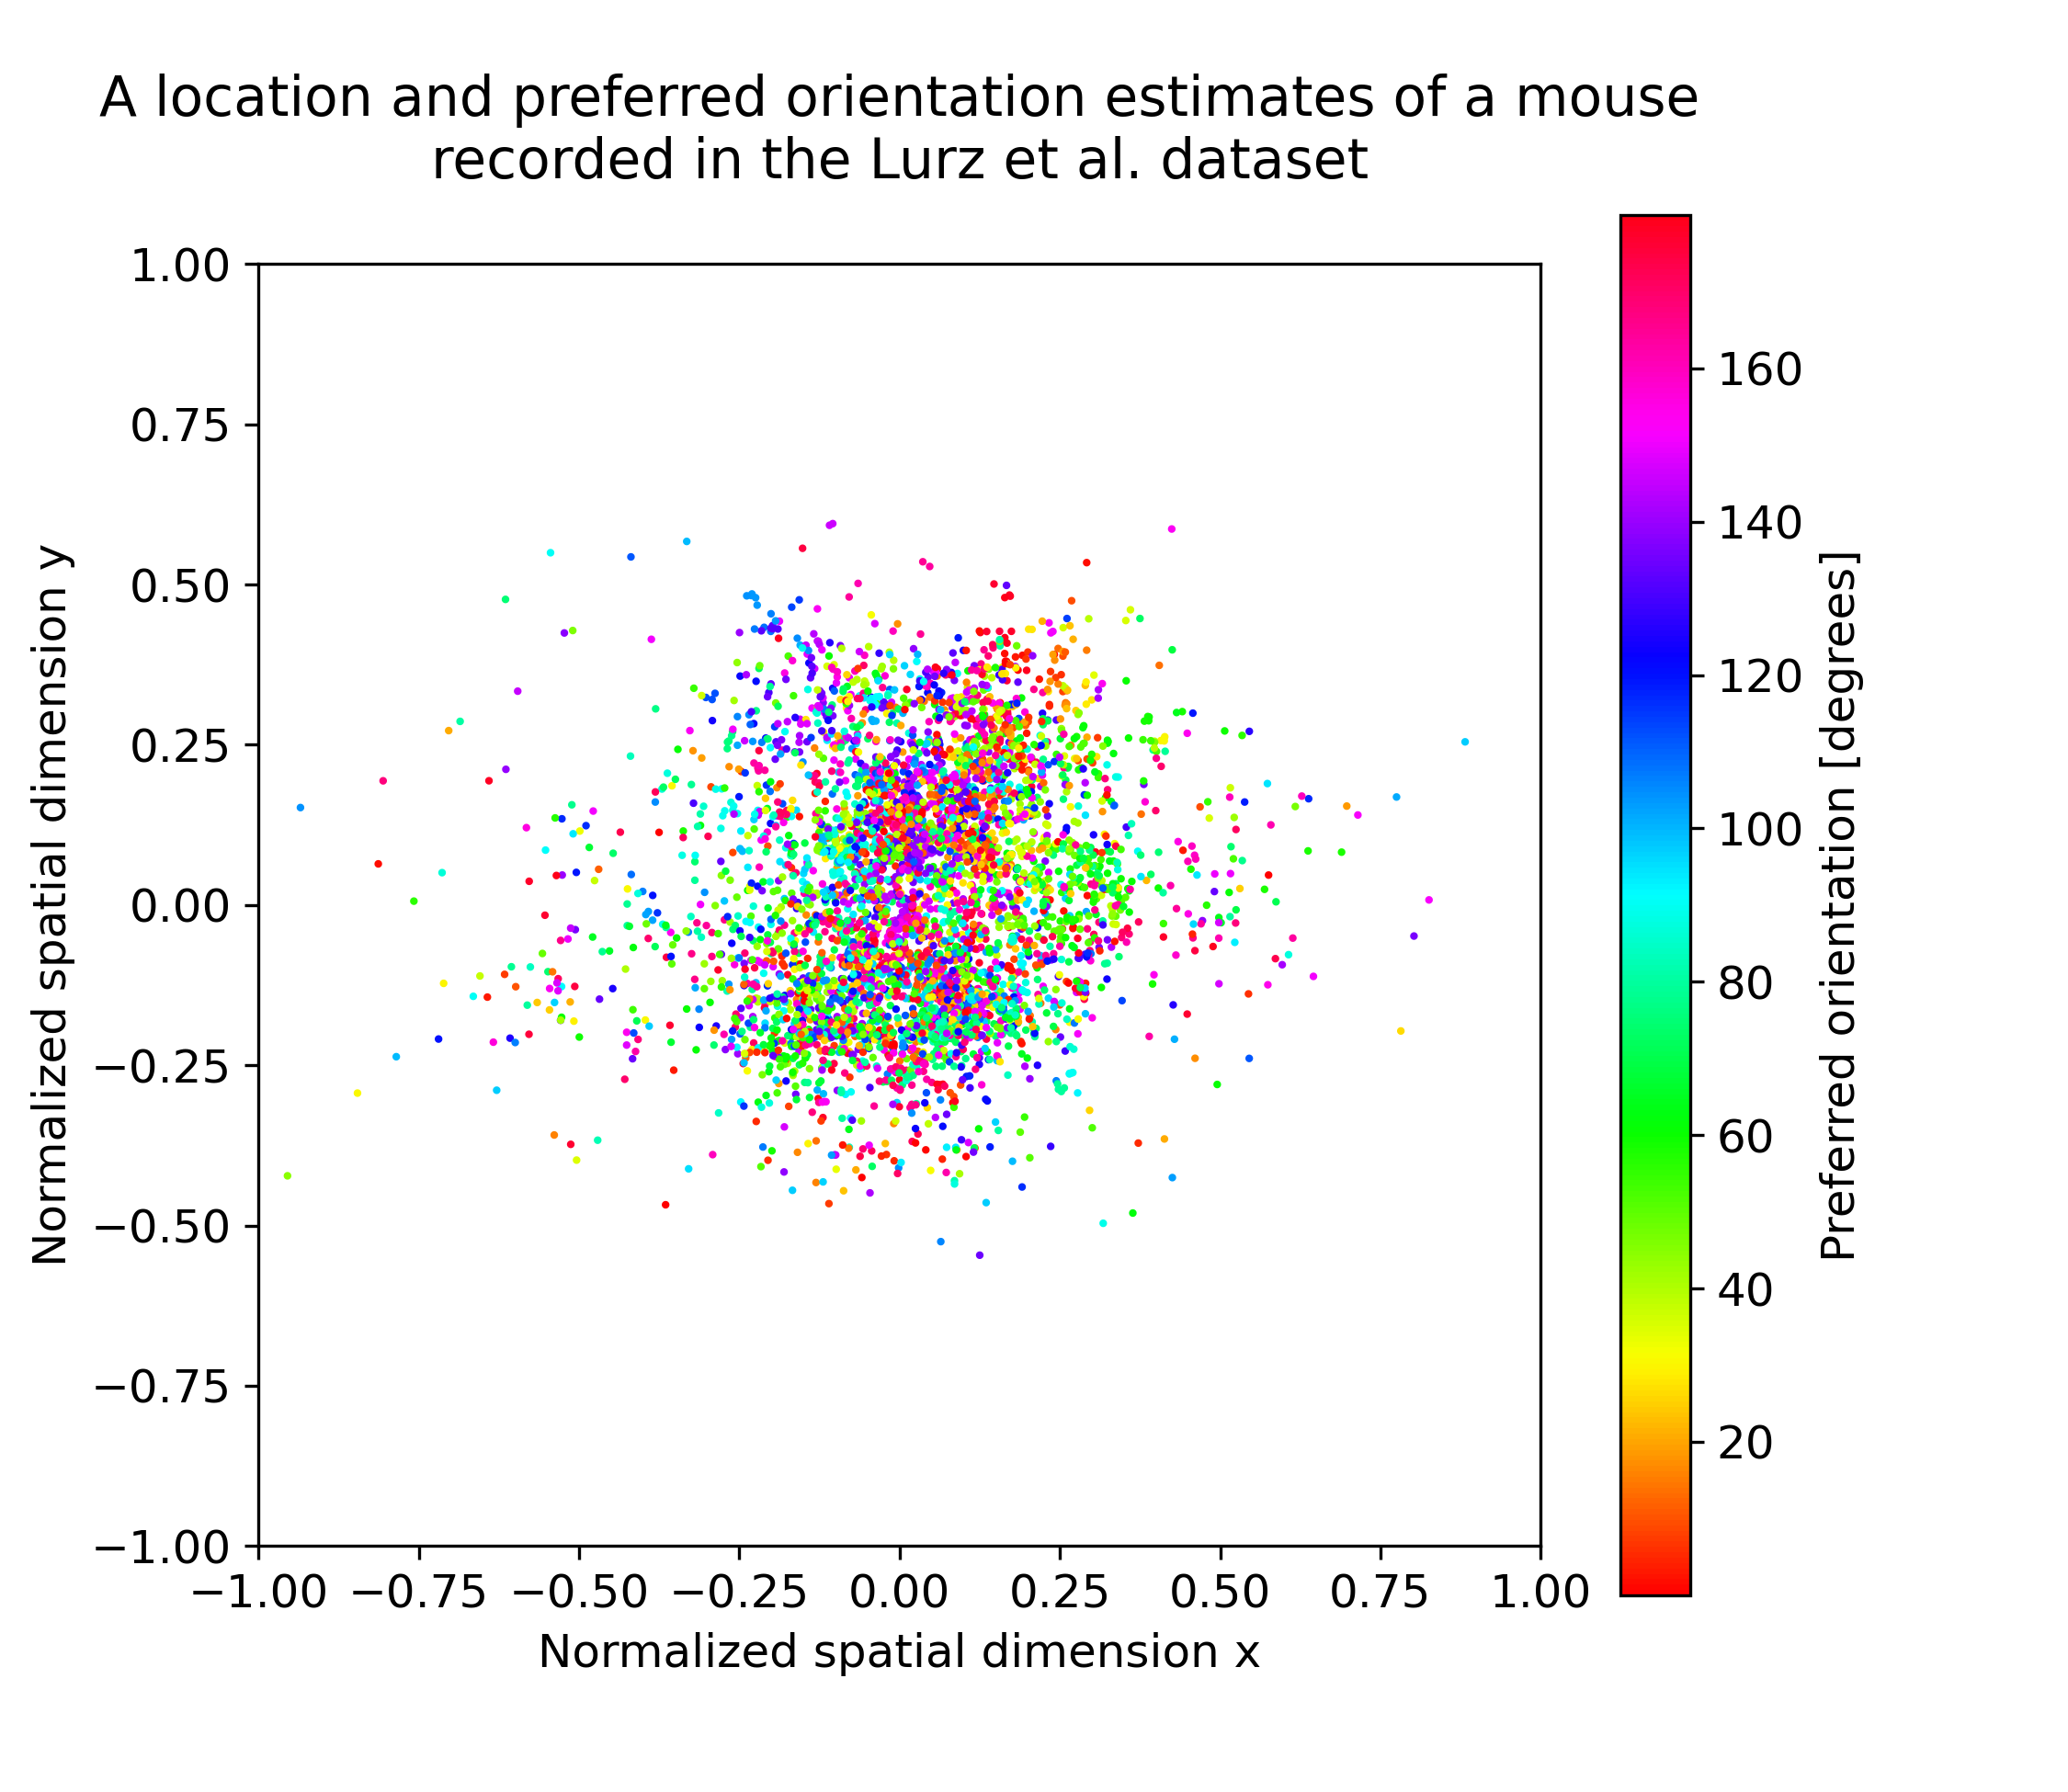
\includegraphics[width=140mm]{../img/reconstructed_orientation_maps_best_lurz.png}
	\caption{A visualization of estimated normalized neural locations along with their orientation preference of the recorded mouse from the dataset from Lurz et al. \citep{lurz2021generalization}. Due to the absence of orientation maps in rodents, the plotted neurons do not exhibit any visible structure.}
	\label{lurz_ori_maps}
\end{figure}

\begin{figure}[H]\centering
	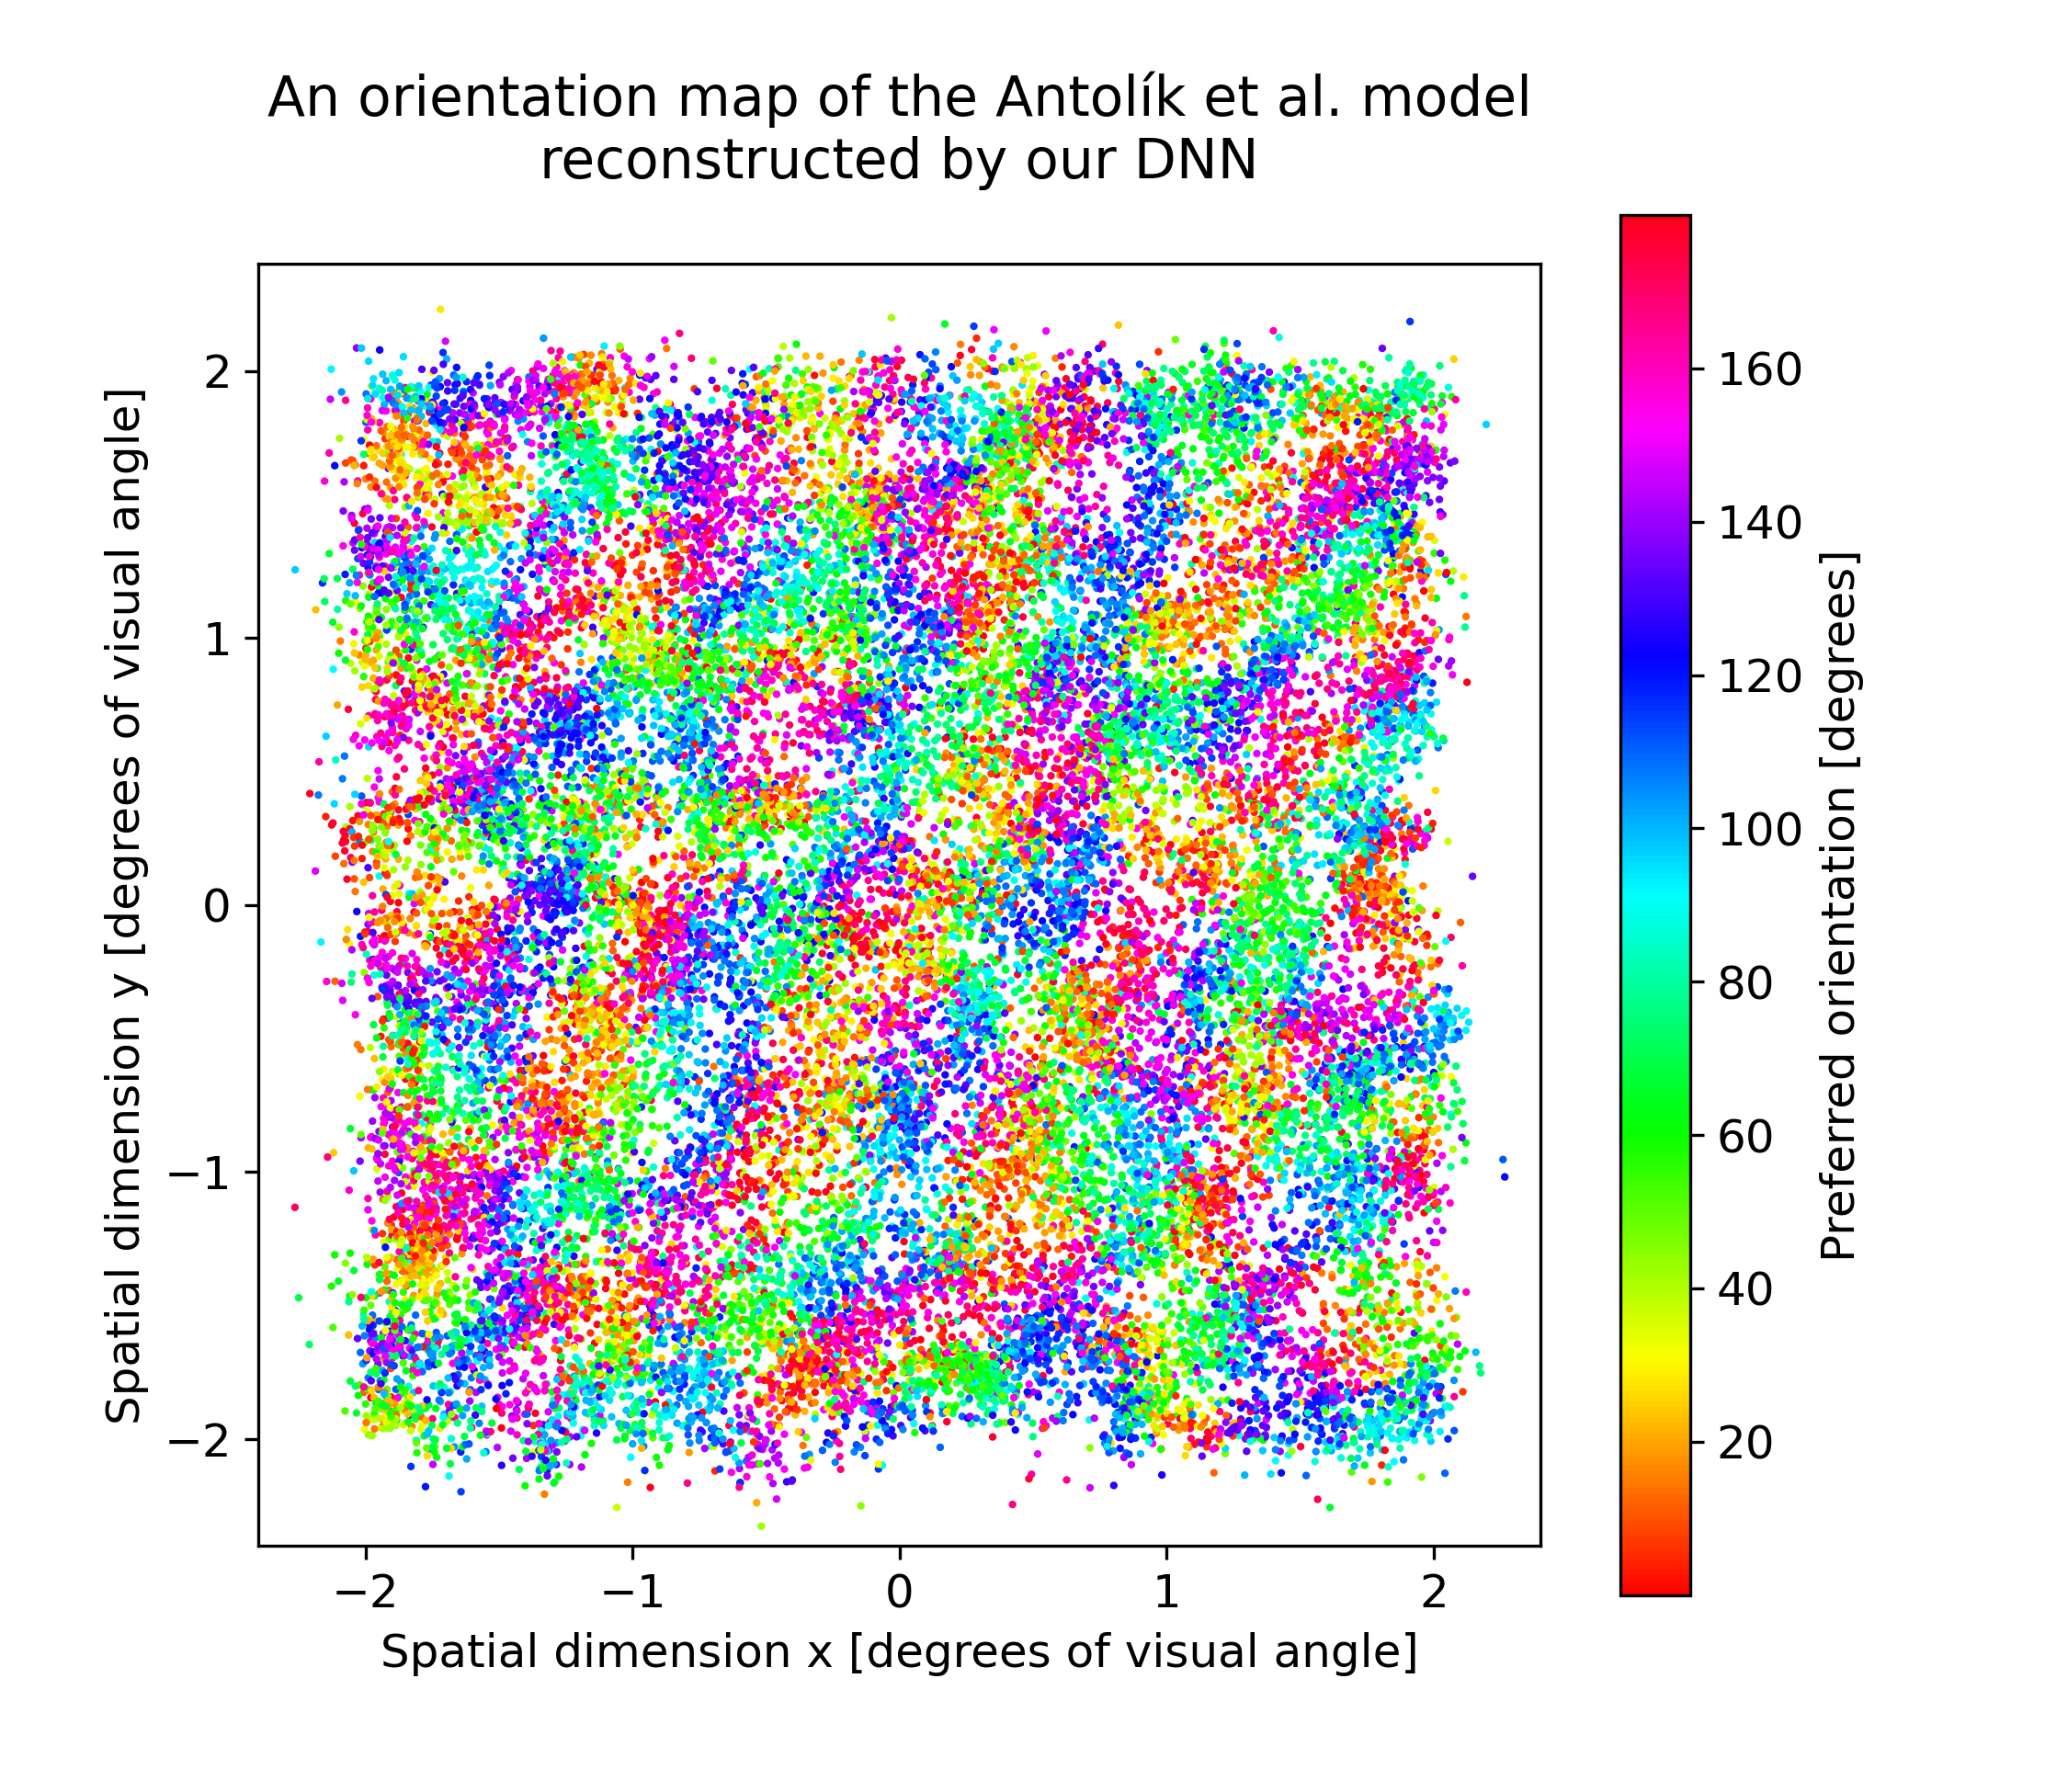
\includegraphics[width=150mm]{../img/reconstructed_orientation_maps_best_antolik.png}
	\caption{The orientation map of the Antolík et al. model \citep{antolik2019comprehensive} reconstructed by our DNN.}
	\label{prediction}
\end{figure}

\begin{figure}[H]\centering
	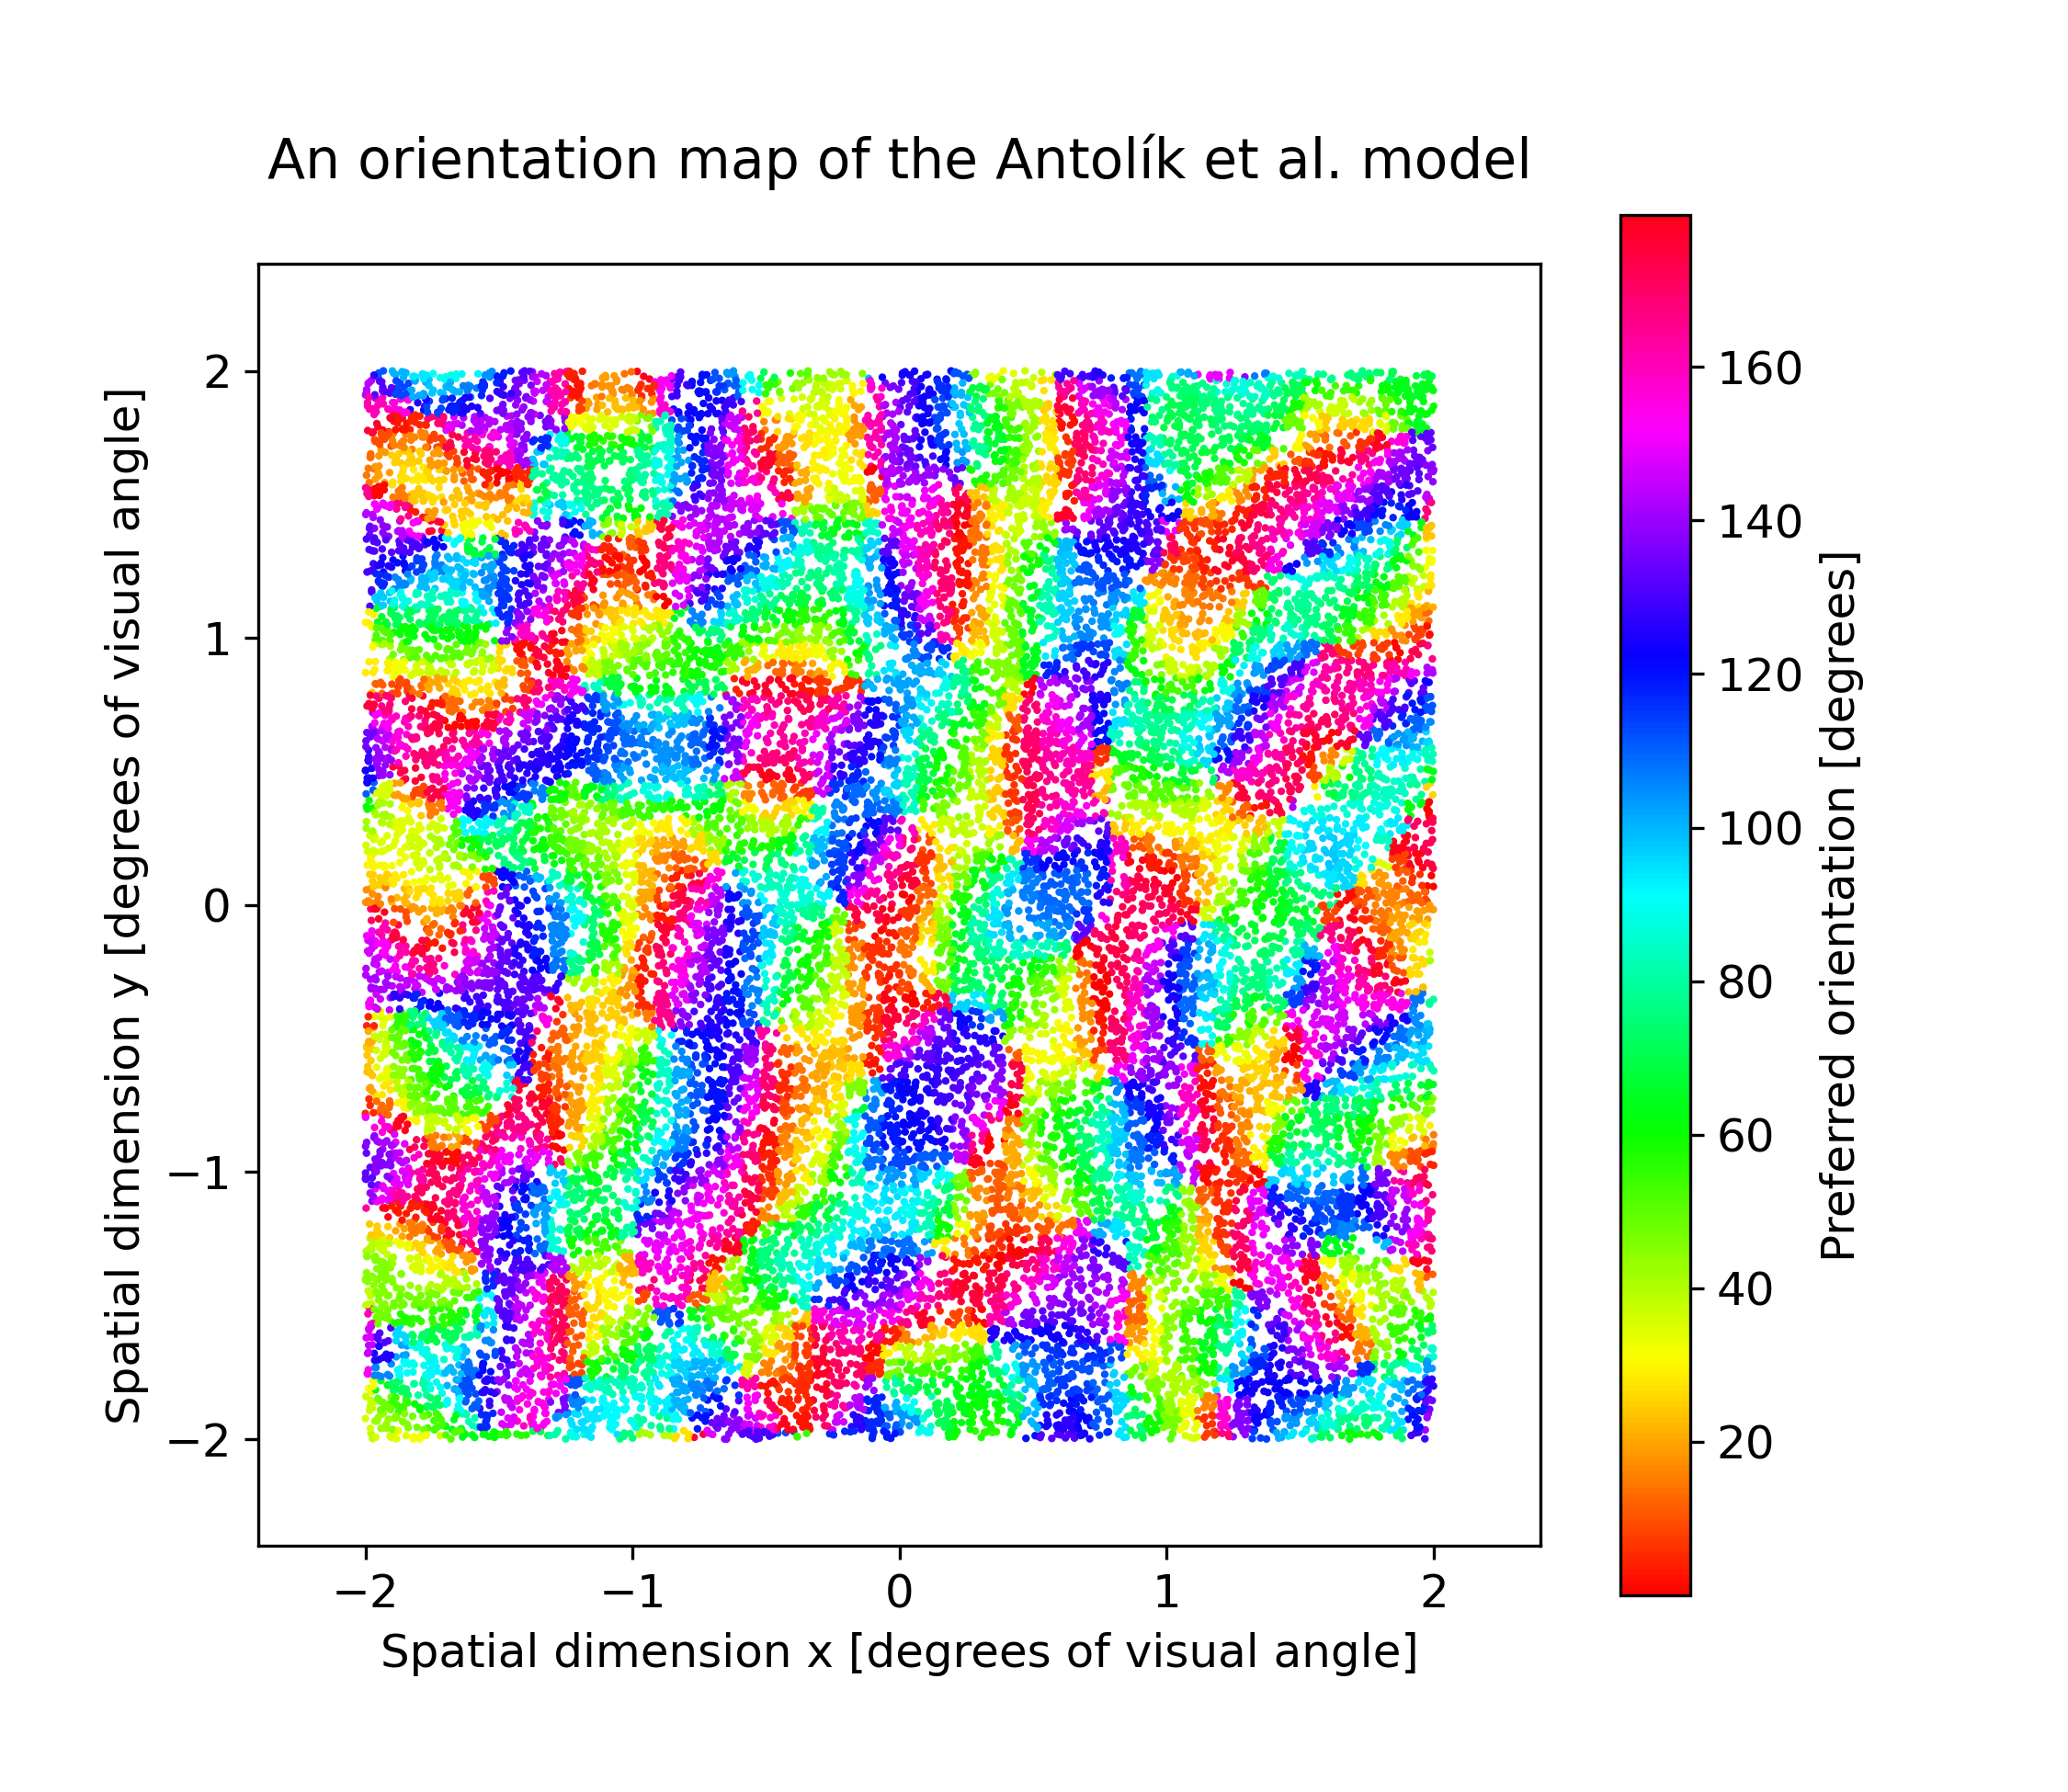
\includegraphics[width=150mm]{../img/reconstructed_orientation_maps_best_truth.png}
	\caption{The original orientation map of the Antolík et al. model \citep{antolik2019comprehensive}.}
	\label{ground_truth}
\end{figure}

The graphical demonstrations contain remarkable similarities in comparing the reconstructed orientation map of the in-silico cat V1 and its available ground truth orientation map (Figure~\ref{ground_truth}). However, to adequately prove that the orientation map reconstruction is accurate, having all necessary data available, we computed the average error in both location and preferred orientation estimates.

To examine the accuracy of the readout estimates in more detail, we plotted the distribution of errors in the neural location prediction (Figure~\ref{err_dist}). A small portion of neurons ($0.16 \%$, in particular, 47~neurons out of an overall 30000) having an estimation error higher than 0.55\,degrees of visual angle were pronounced to be outliers and disregarded in the figure not to pollute the visualization of the error distribution. Surprisingly, the average error is small; only 0.1\,degrees of visual angle.

\begin{figure}[H]\centering
	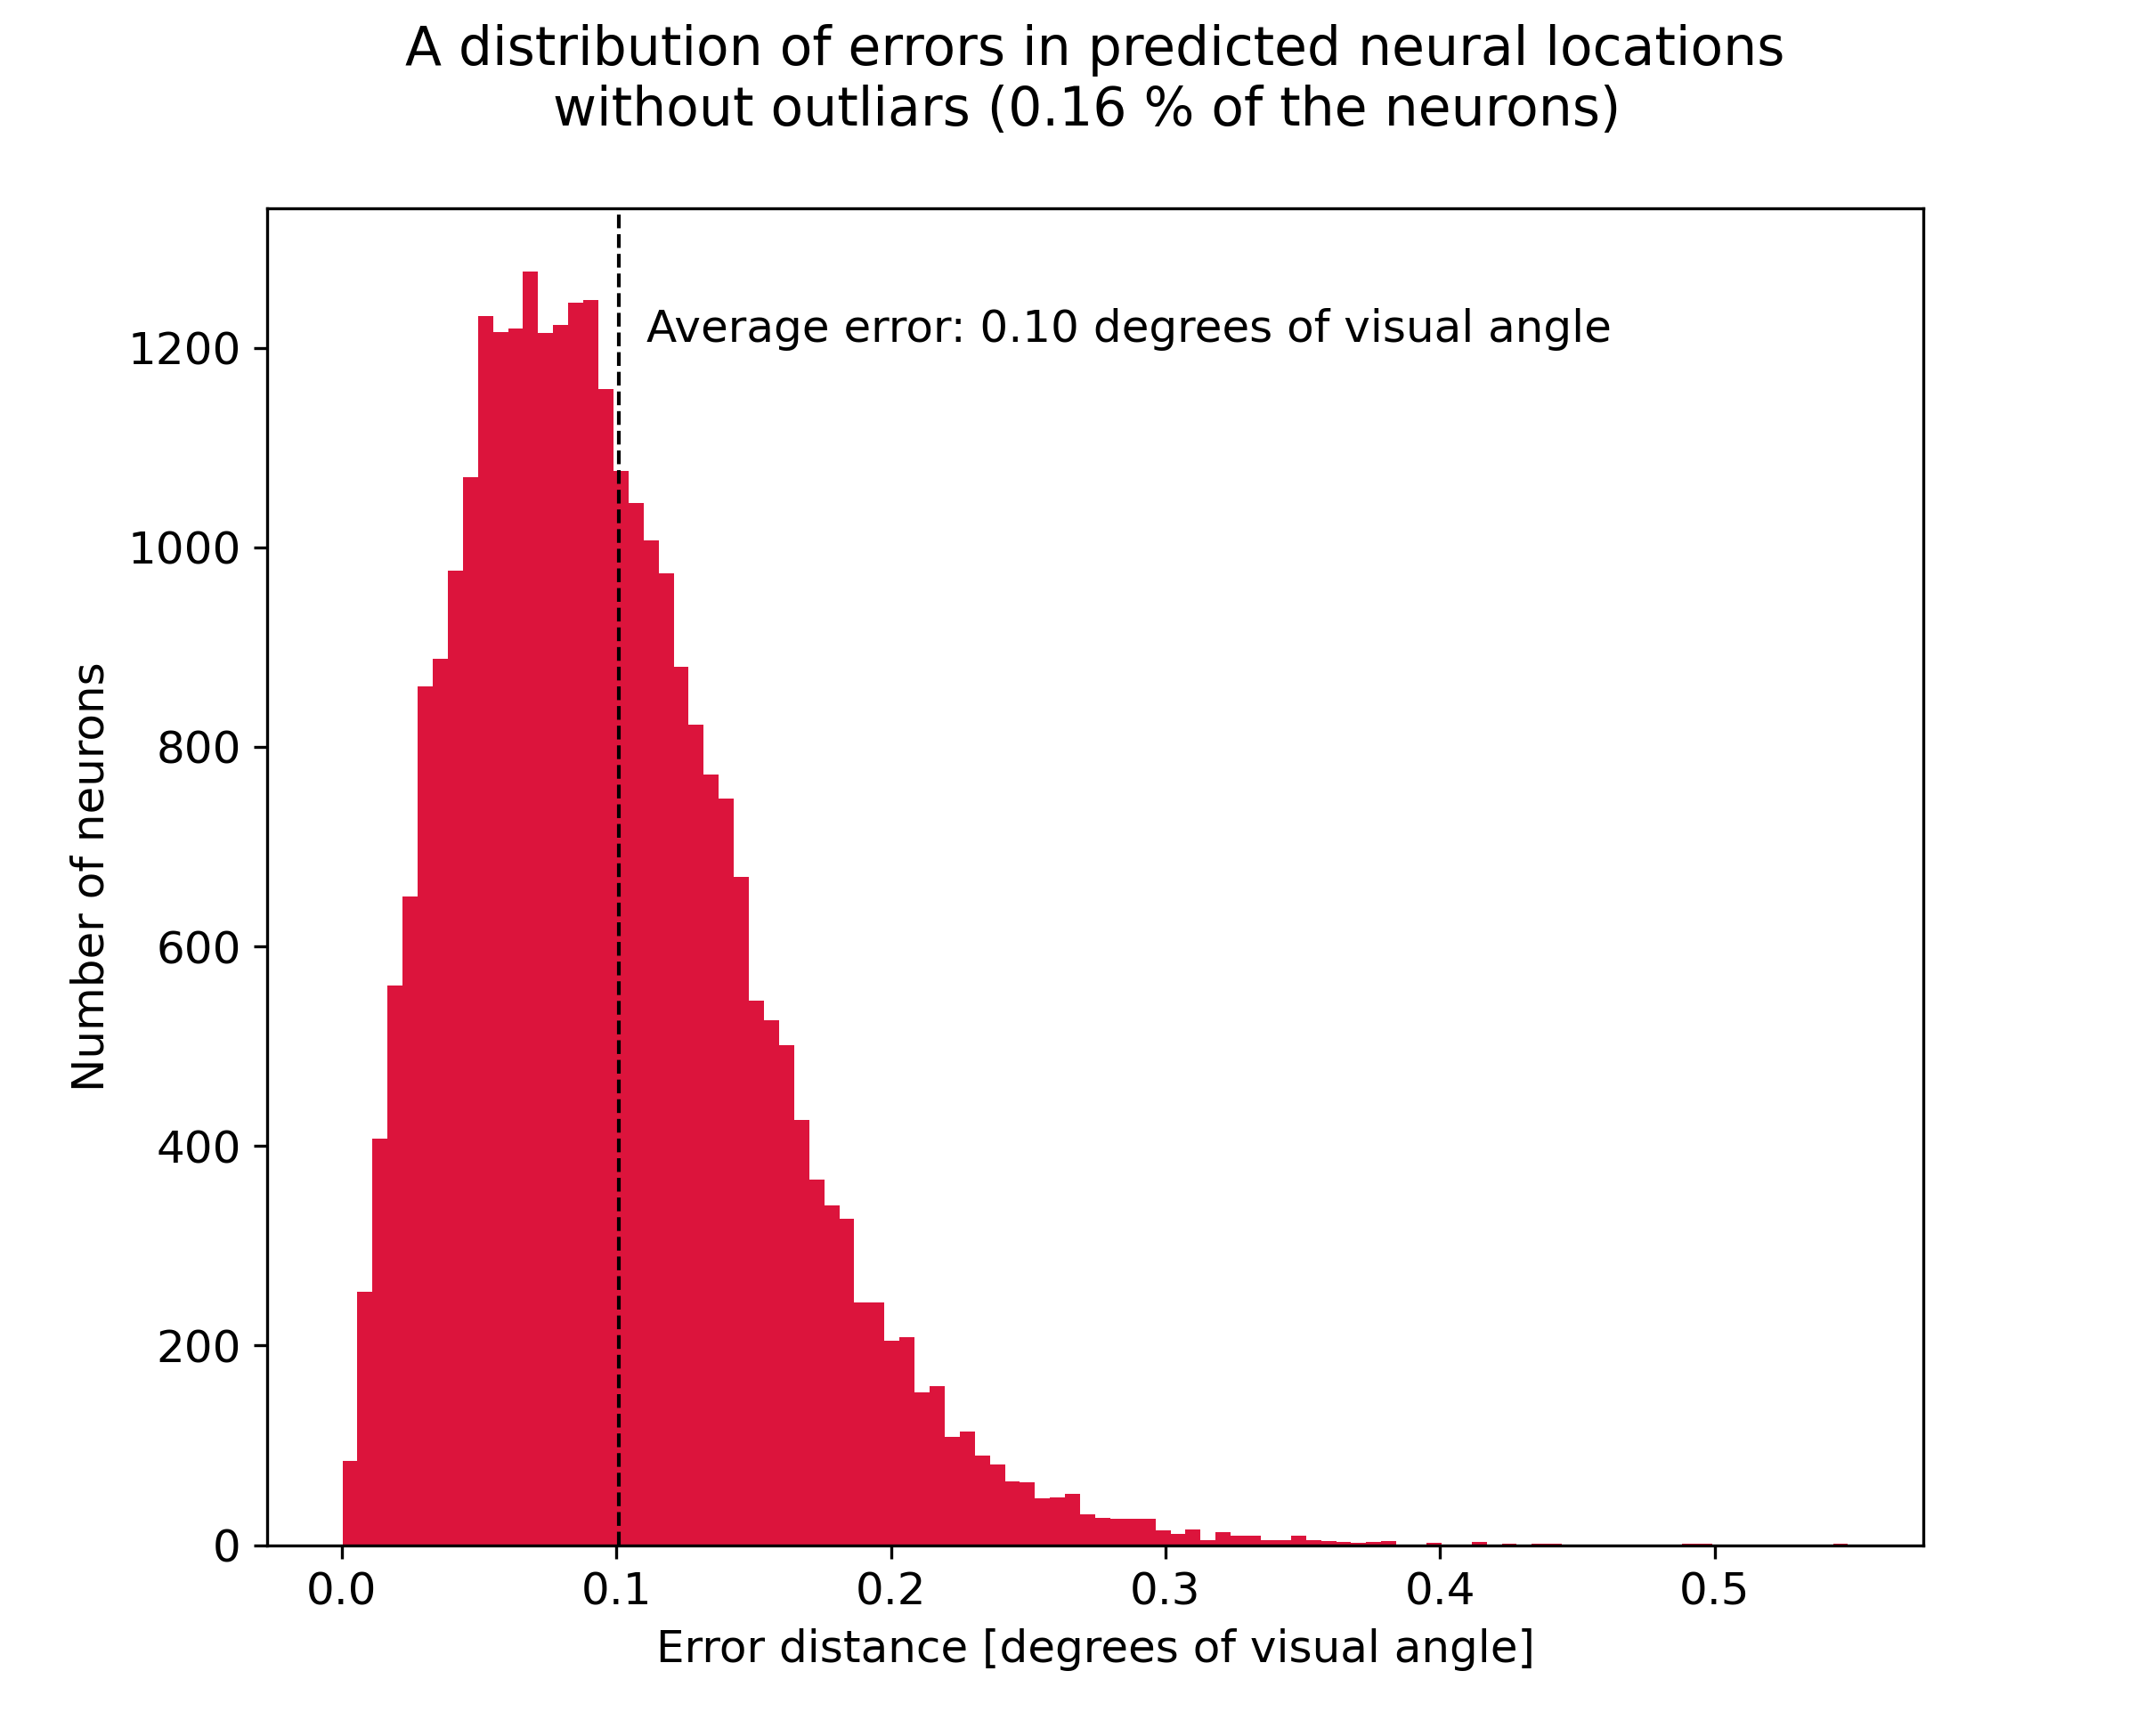
\includegraphics[width=150mm]{../img/distribution_of_distances_errors.png}
	\caption{A distribution of errors in predicted neural locations that disregards 47 outlying neurons ($0.16 \%$) to not pollute the visualization.}
	\label{err_dist}
\end{figure}


Furthermore, we investigated the orientation preference estimates. In comparison to the predicted location, the average error is comparably higher, yielding the value of 15.93\,degrees. In Figure~\ref{err_ori} we present the graphical depiction of the distribution of errors in orientation preference estimates.

\begin{figure}[H]\centering
	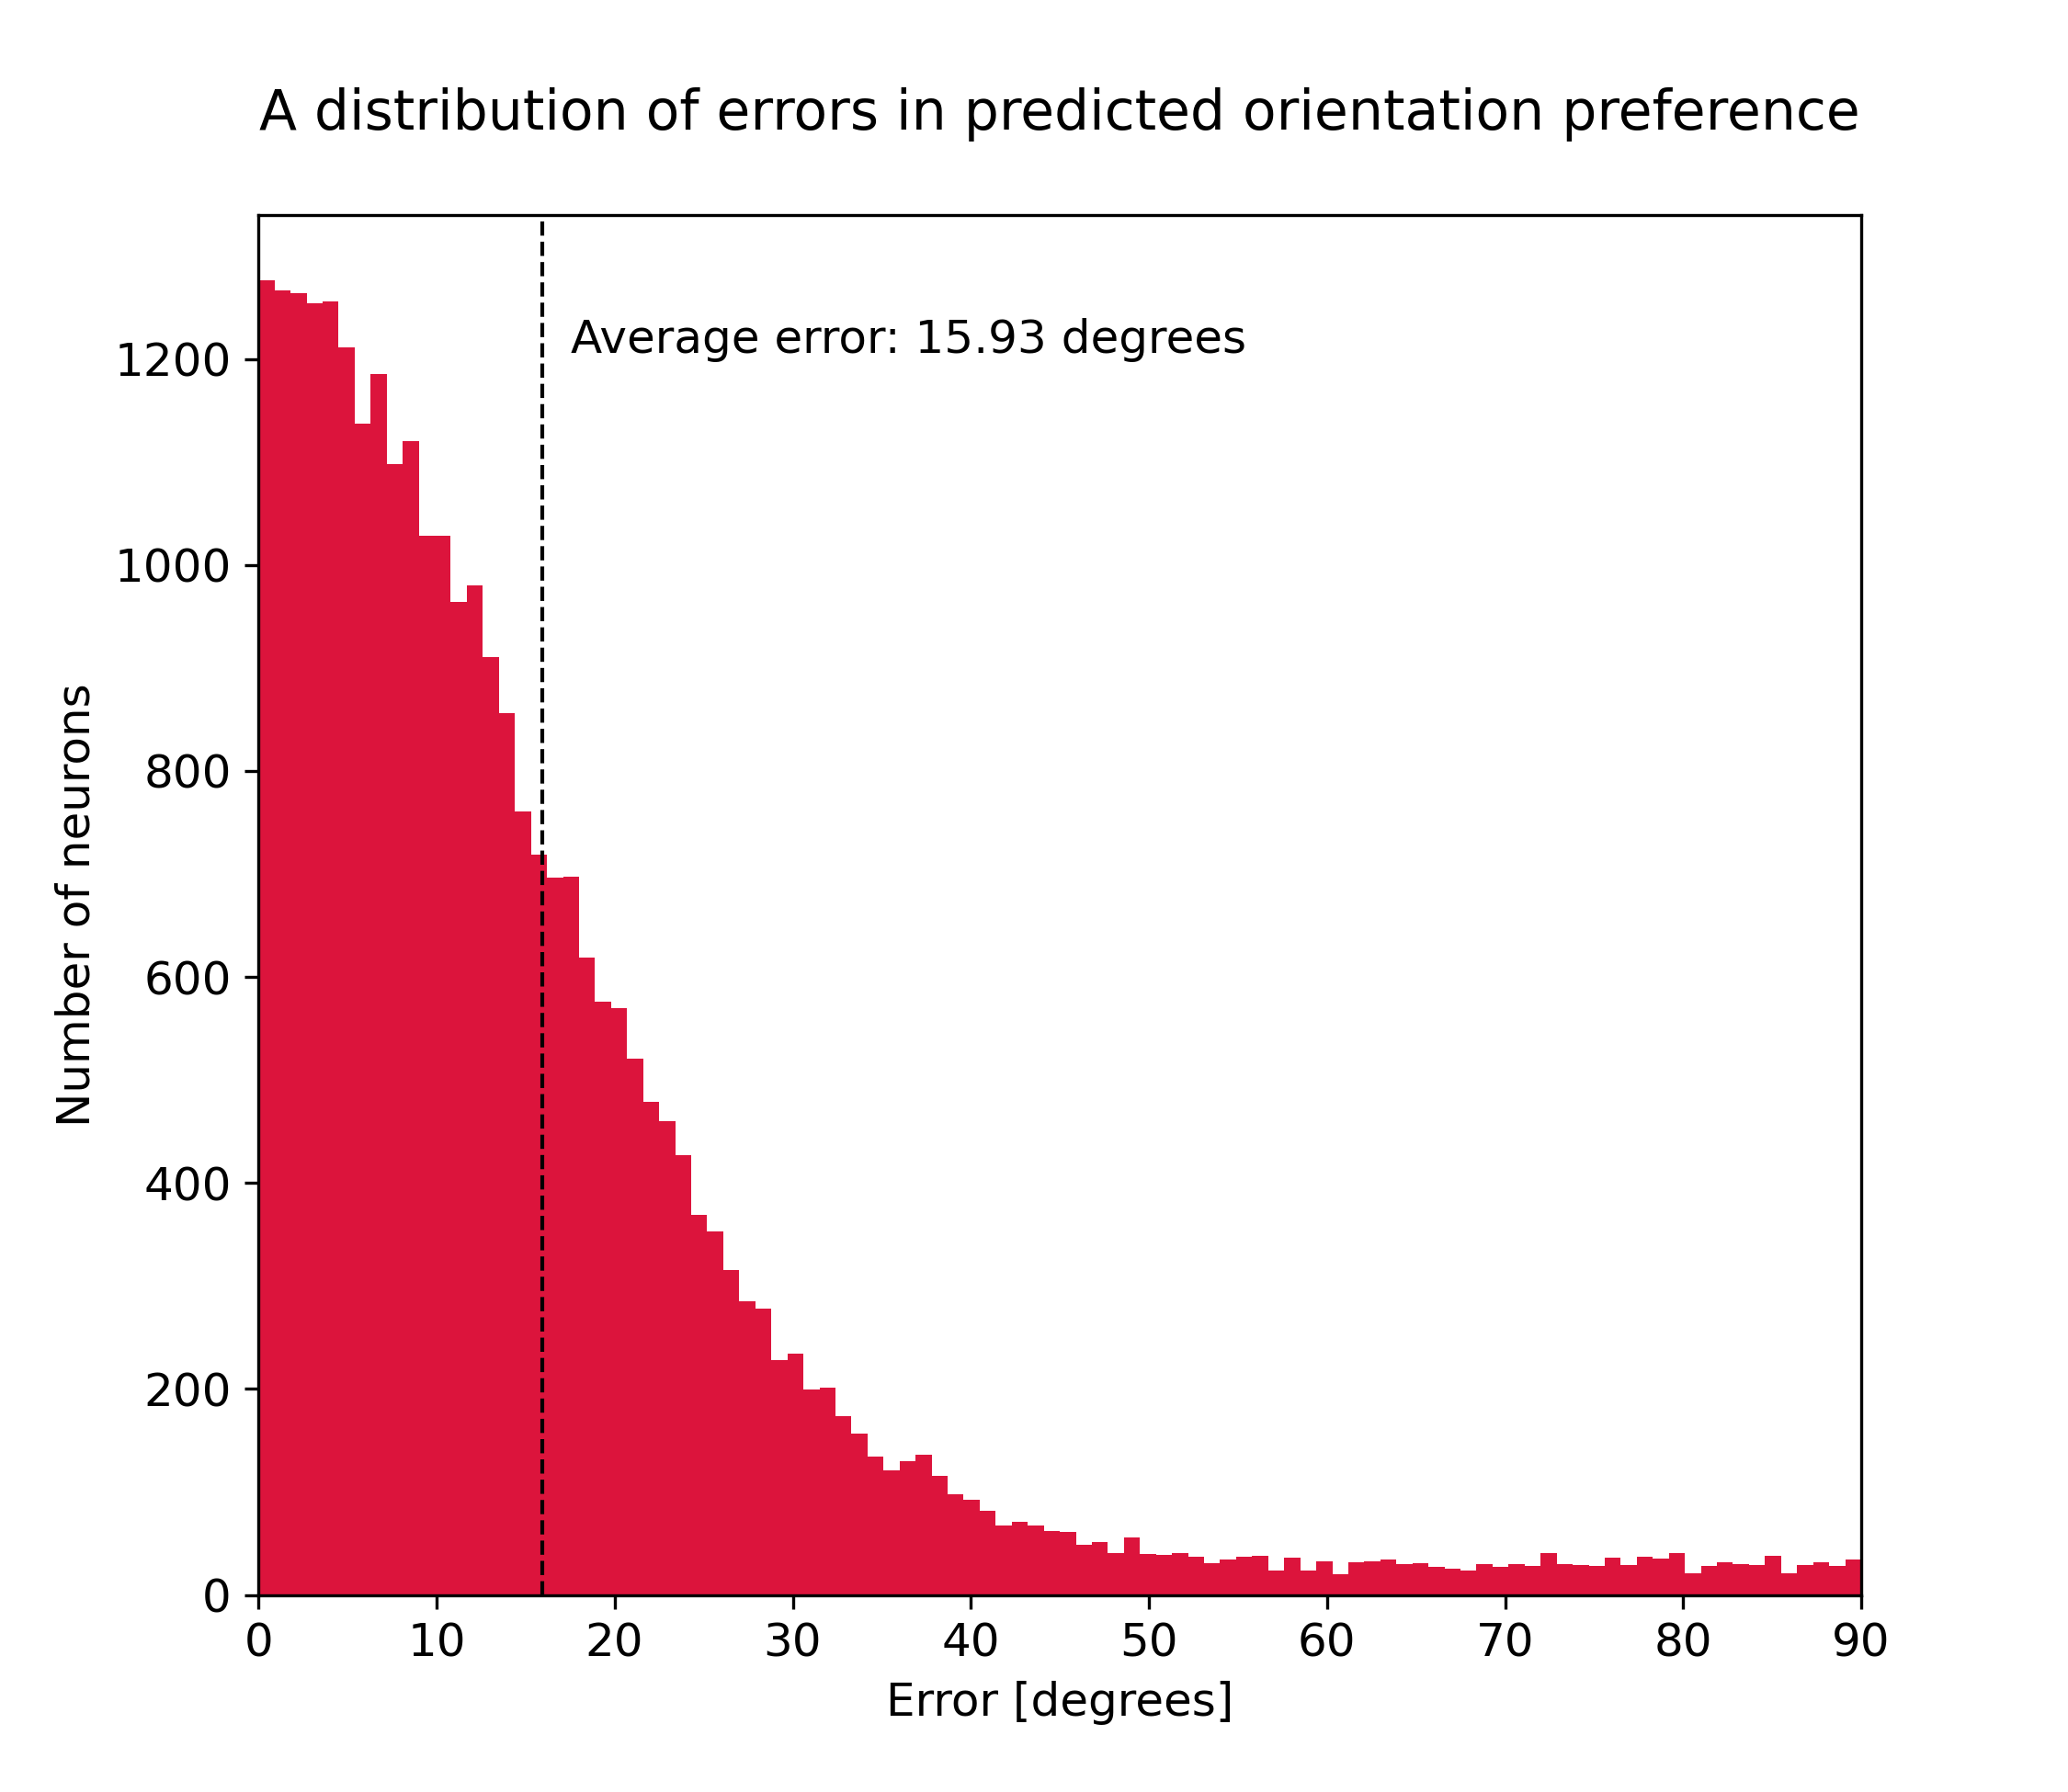
\includegraphics[width=150mm]{../img/distribution_of_orientation_errors.png}
	\caption{A distribution of errors in orientation preference estimates. The average error is higher compared to the error in location estimates. For a very small portion of neurons, the orientation is, however, not learned at all.}
	\label{err_ori}
\end{figure}

























